\documentclass[12pt]{Report}
\usepackage{graphicx}
\usepackage{listings}

\usepackage{verbatim} 

\begin{document}
\title{Assignment 2 : CS 751 }
\author{HARISH}

\maketitle

\section{Part 1}

\paragraph{Choose 100 URIs from A1
Generate WARC files of those URIs using:wget,WARCreate,Heritrix (stand-alone or via WAIL),webrecorder.io}

\subparagraph{WARC using webrecorder.io}


I have chosen 100 URIs from Assignment1. In order to generate WARC files in webrecorder.io , we use "https://webrecorder.io/" and record the data using the options provided in the website . The WARC for all the 100 URIs are generated . It can be downloaded in zip format . The file 100interestingurlss.txt contains the 100 urls.

\subparagraph{WARC using WARCreate}

The WARC files using WARCreate can be achieved via chrome plugin 'WARCreate' . The WARC files are downloaded in zipped format (.gz).

\subparagraph{WARC using wget }

I have written a shell script using wget command to download warc files for all the URIs . 

\subparagraph{WARC using WAIL}

I have used following steps to set up WAIL in the system.


1. Install application from webpage, download: Windows 7+, version 0.2013.2.19 \\
2. Unzip \\
3. Install wx python module: http://www.wxpython.org/download.php (I installed the last one 64-bit, python 2.7) \\
4. Moved "WAIL..." to C:\ and rename "WAIL" (remove extra characters) \\
5. Moved every file folder to the path C:WAIL (That is make direct path to folder, no intermediate folders) \\
6. Modified BDBCollection.xml as mentioned in google groups.\\
7. In WAIL.py changed catalina-start.bat . \\


I followed the below step for adding multiple URIs to WAIL , to crawl all links at once \\

WAIL : Advanced : Setup One-Off Crawl : Click first line to add URI0  : Click first line to add URI1 ... : Clicked Launch Crawl \\


\subsubsection{WAIL Instance}
\begin{figure}[ht]    
    \begin{center}
        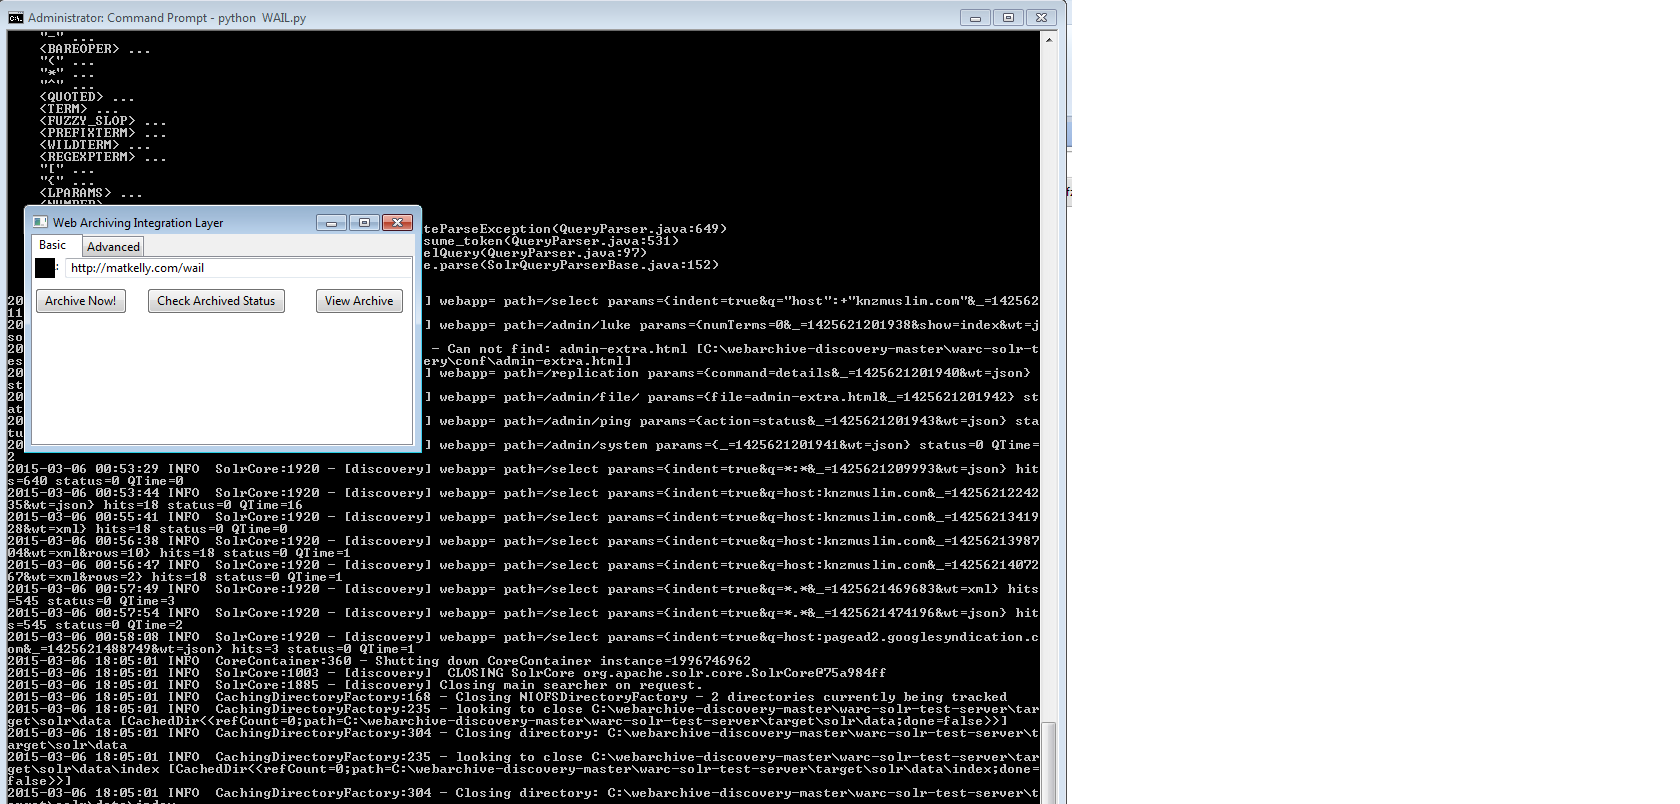
\includegraphics[scale=0.60]{wailinstance.png}
        \caption{Web Archiving Integration Layer }
        \label{warc file size comparision}
    \end{center}
\end{figure}
\newpage



\paragraph{Describe the resulting WARC files: quantitatively compare and contrast the results of the WARC files of the same URI as generated by different tools }

In order to quantitatively compare and contrast the results of the WARC files , I have taken 2 URIs and compared their warc file size generated by 4 different tools. \\
I have created a bar plot which contains the size differences of the warc files for same URIs. I have also pasted the Rscript(sizeComparision.R located in the same folder) which i have used to plot this graph . 
 


\newpage
\subsubsection{File Size Comparison}
\begin{figure}[ht]    
    \begin{center}
        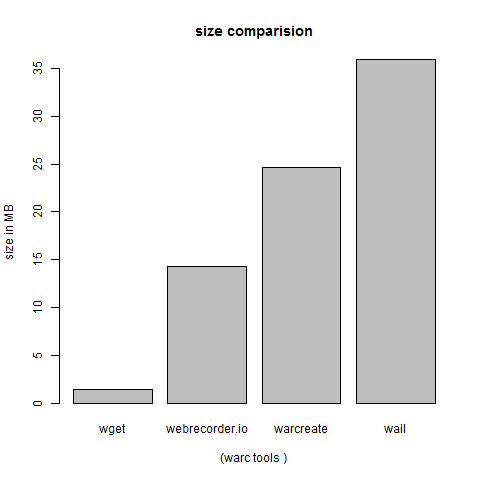
\includegraphics[scale=0.60]{warcsizeComparision1.png}
        \caption{warc size comparison 1}
        \label{warc file size comparision}
    \end{center}
\end{figure}
\newpage
\begin{figure}[ht]    
    \begin{center}
        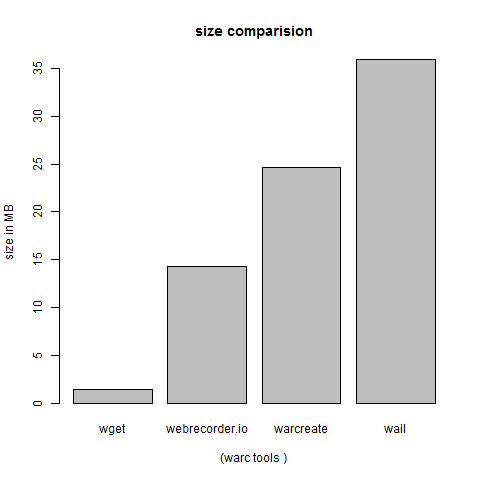
\includegraphics[scale=0.60]{warcsizeComparision1.png}
        \caption{Histogram 2}
        \label{warc file size comparision}
    \end{center}
\end{figure}
\newpage


The size of same URI warc file depends on the tool we use to generate it . WAIL warc size is comparatively long when compared to other warc file tools because wail crawls for the links present in the URI and gets the data of those links as well. wget warc file size is comparatively smaller than other warc files size. 



\paragraph{Demonstrate playback of 2-3 WARCs in the (Wayback Machine (via WAIL or stand-alone) or pywb) and (webrecorder.io)
} 


I have played the same WARC file using pywb and webrecorder.io. 

I have used this link to setup pywb ''https://github.com/ikreymer/pywb ''.
Pywb takes the warc and uses the following command to generate cdx file.\\

''cdx-indexer --sort myarchive/cdx myarchive/warcs''


After setting up pywb . Run the wayback server using wayback command .We can search for the URIs using "http://localhost:8080/pywb"




I have  included playback screen shots generated using pwyb(Figure 4,5 ) .Also ,I have included the playback screen shots generated using webrecorder.io ( Figure 6 , 7 ,8)

\newpage
\begin{figure}[ht]    
    \begin{center}
        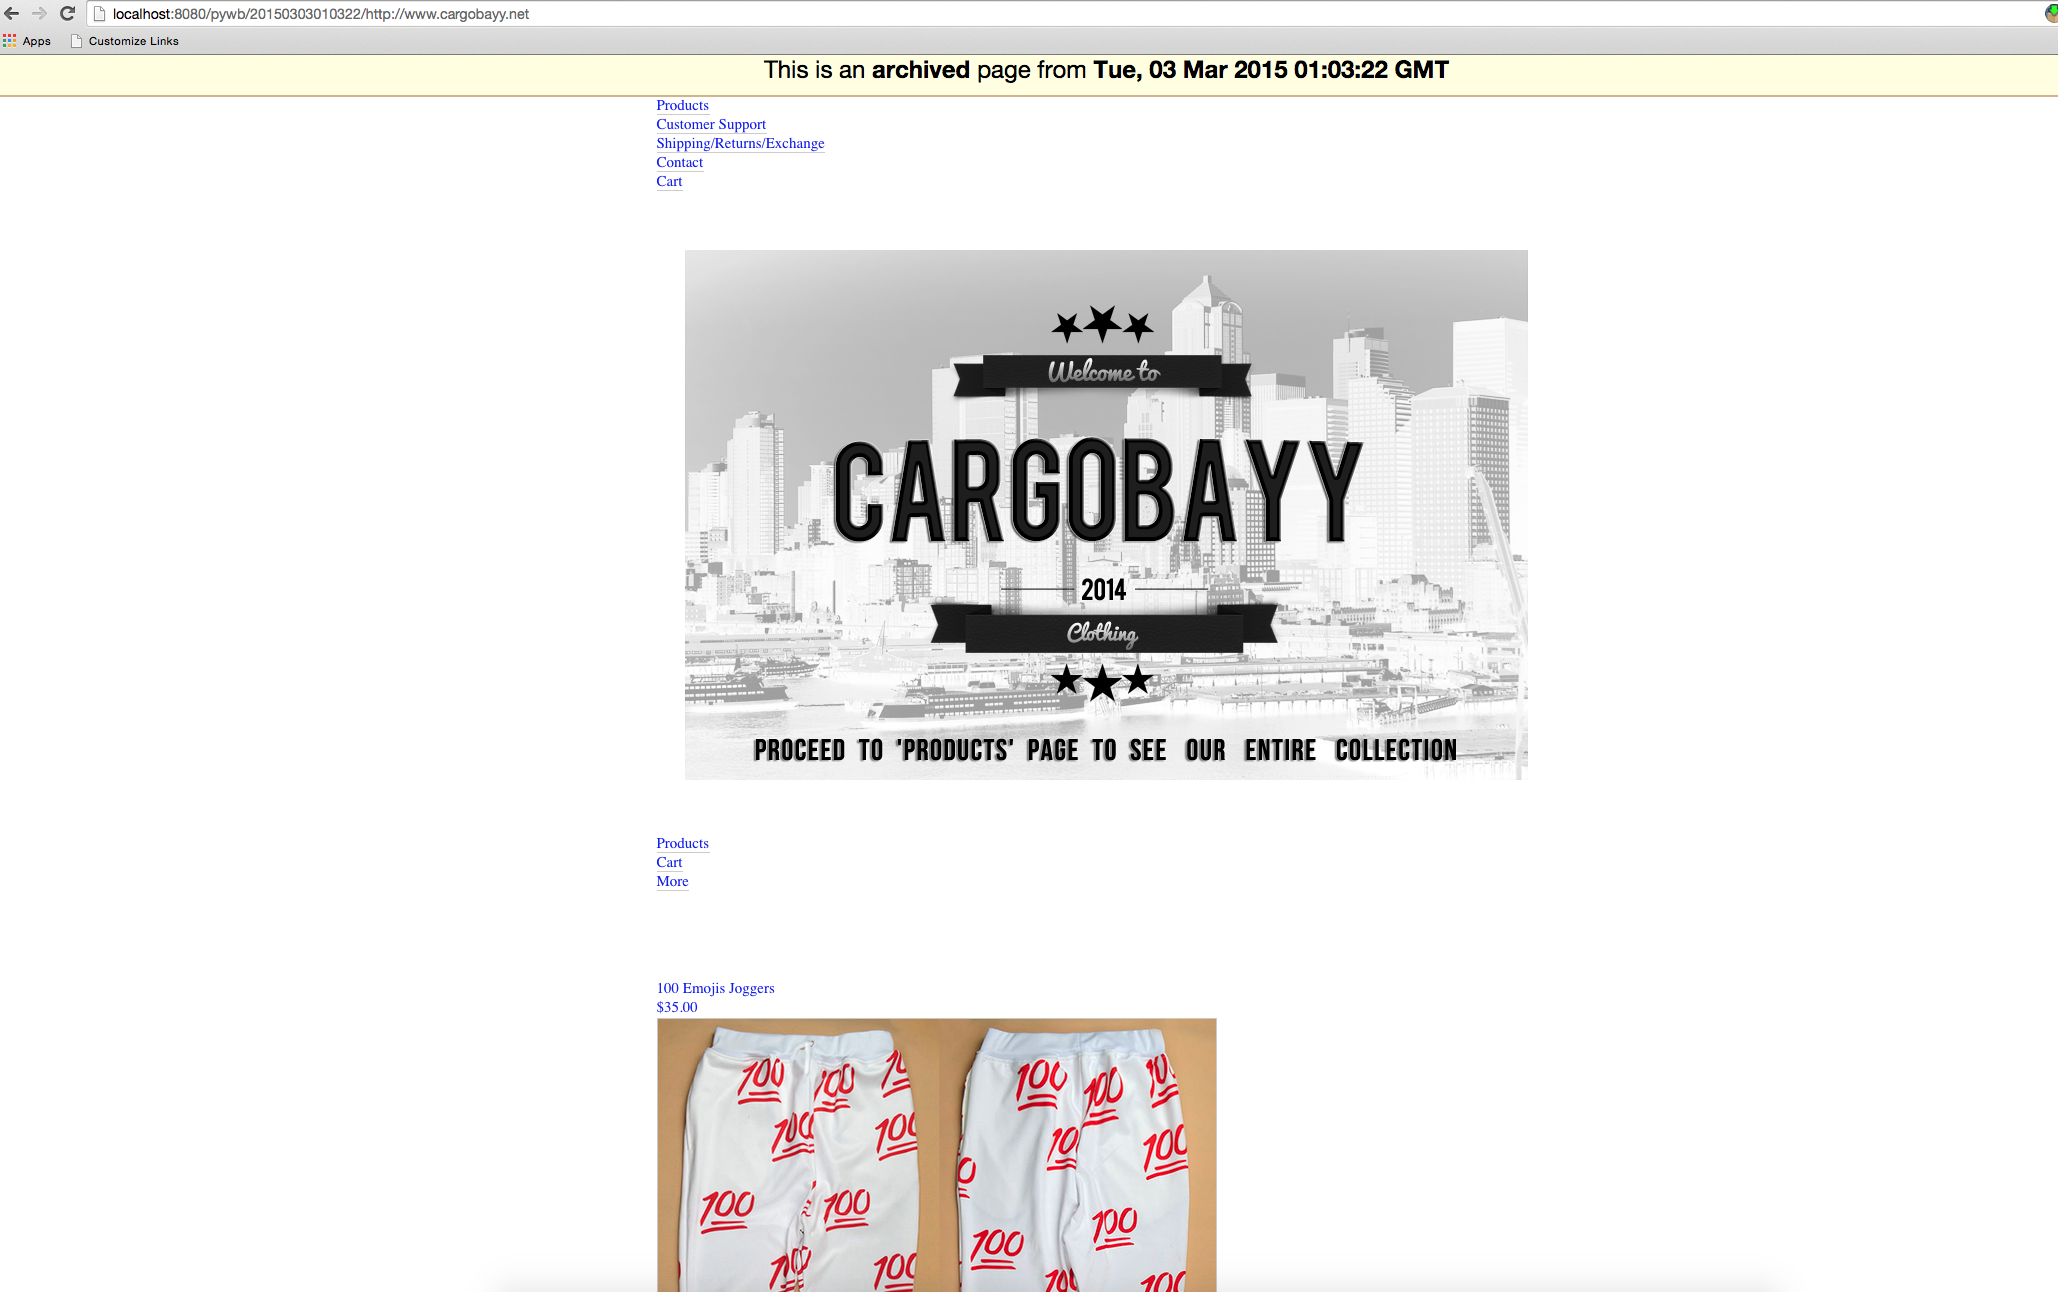
\includegraphics[scale=0.60]{pywb1.png}
        \caption{playback 1}
        \label{pywb playback}
    \end{center}
\end{figure}
\newpage
\begin{figure}[ht]    
    \begin{center}
        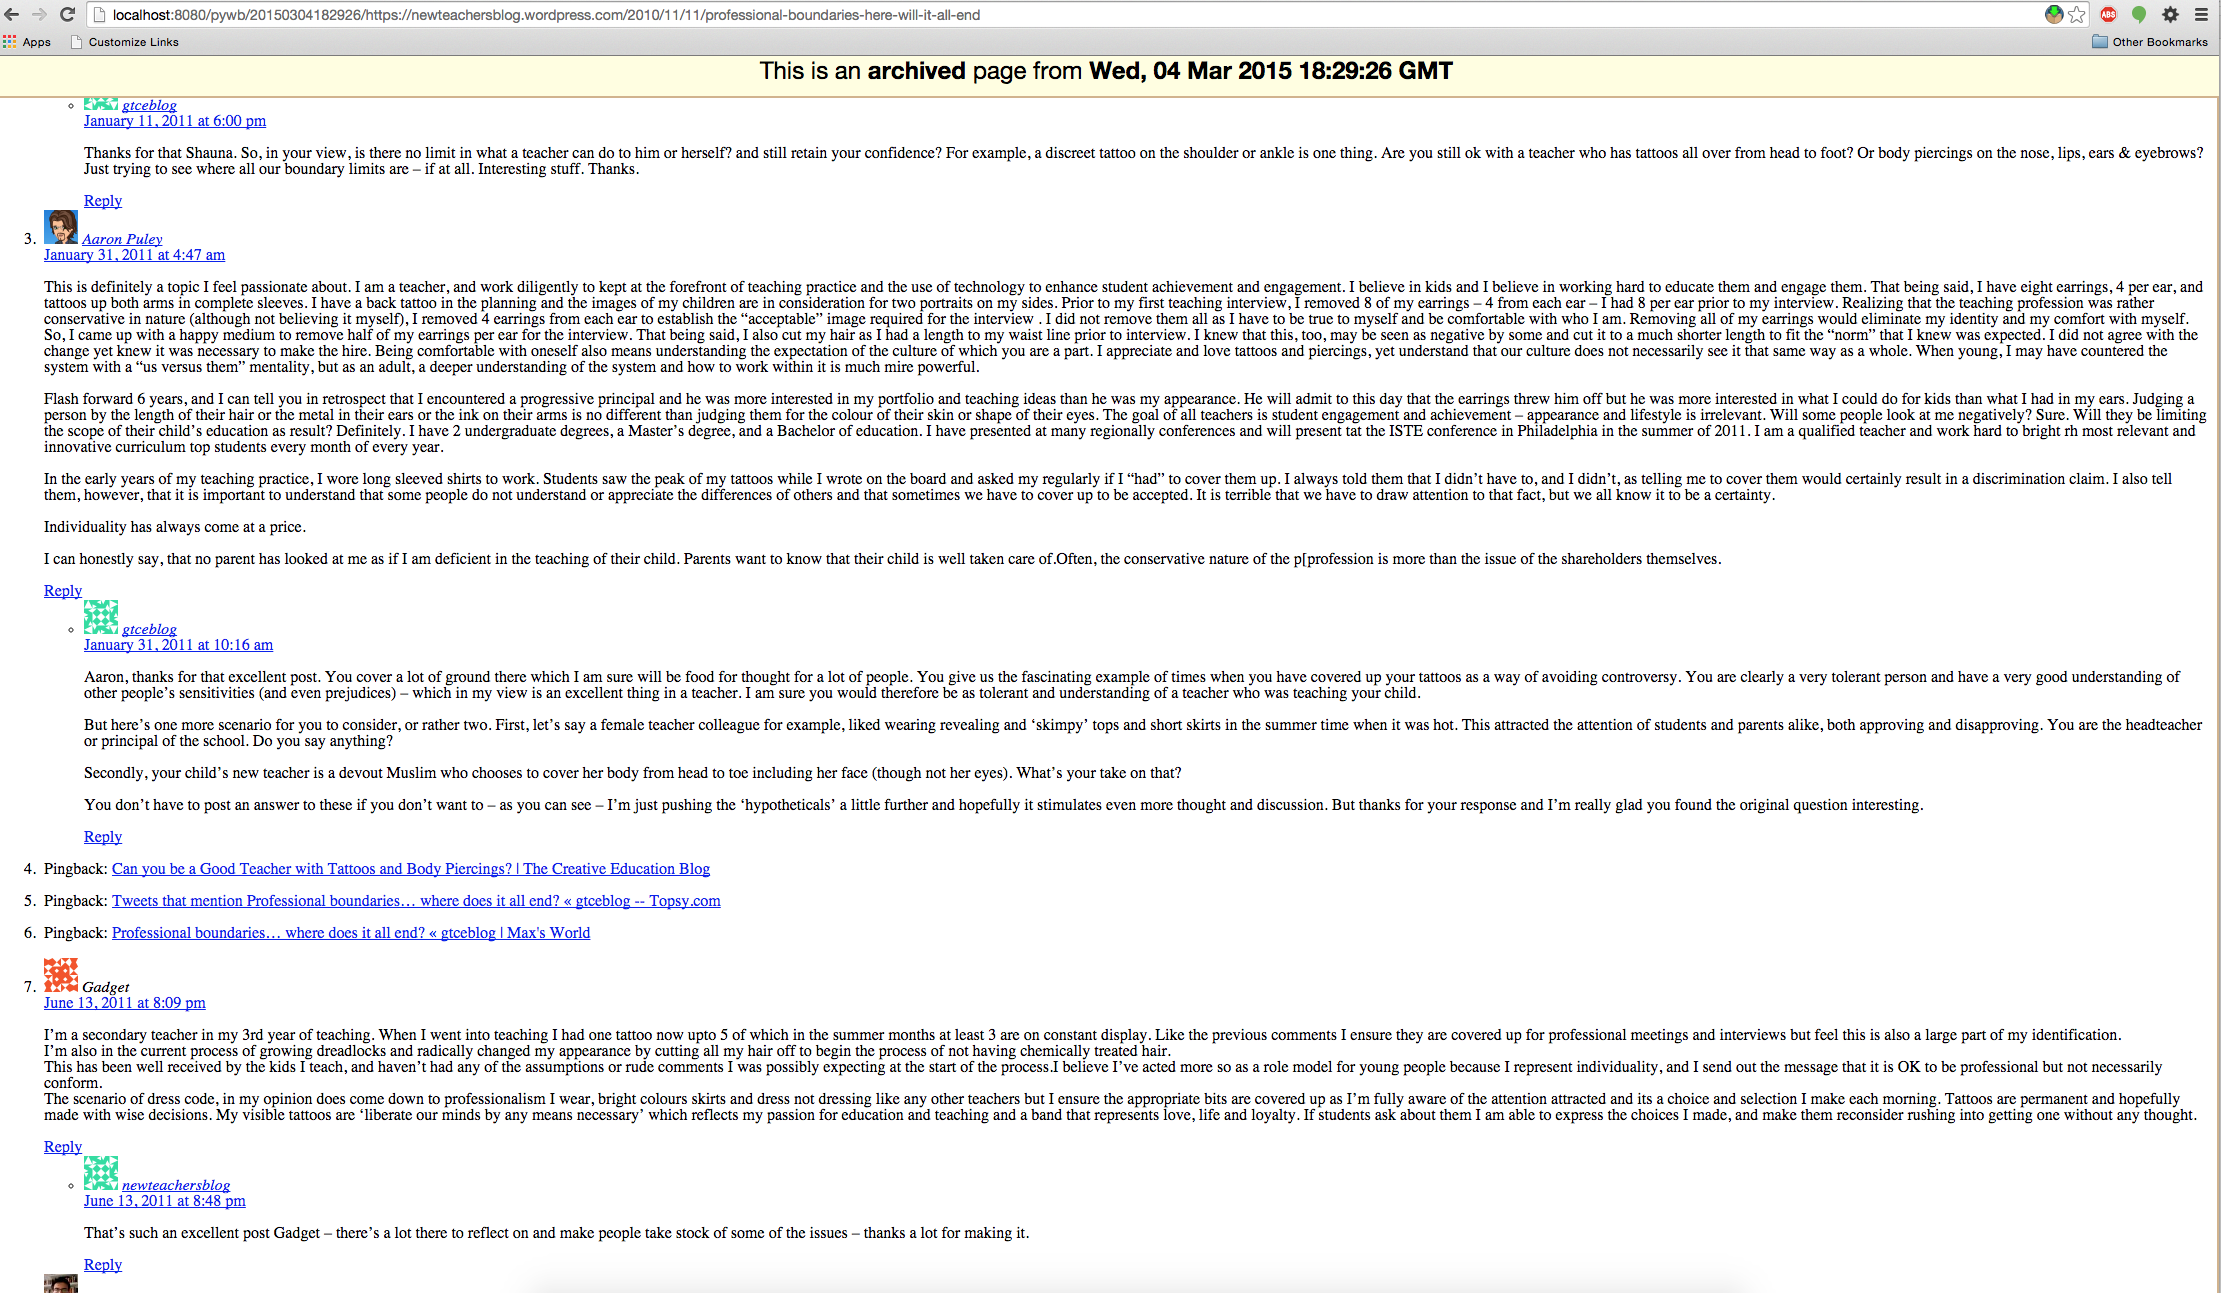
\includegraphics[scale=0.60]{pywb2.png}
        \caption{playback 2}
        \label{pywb playback}
    \end{center}
\end{figure}
\newpage



 

\newpage
\begin{figure}[ht]    
    \begin{center}
        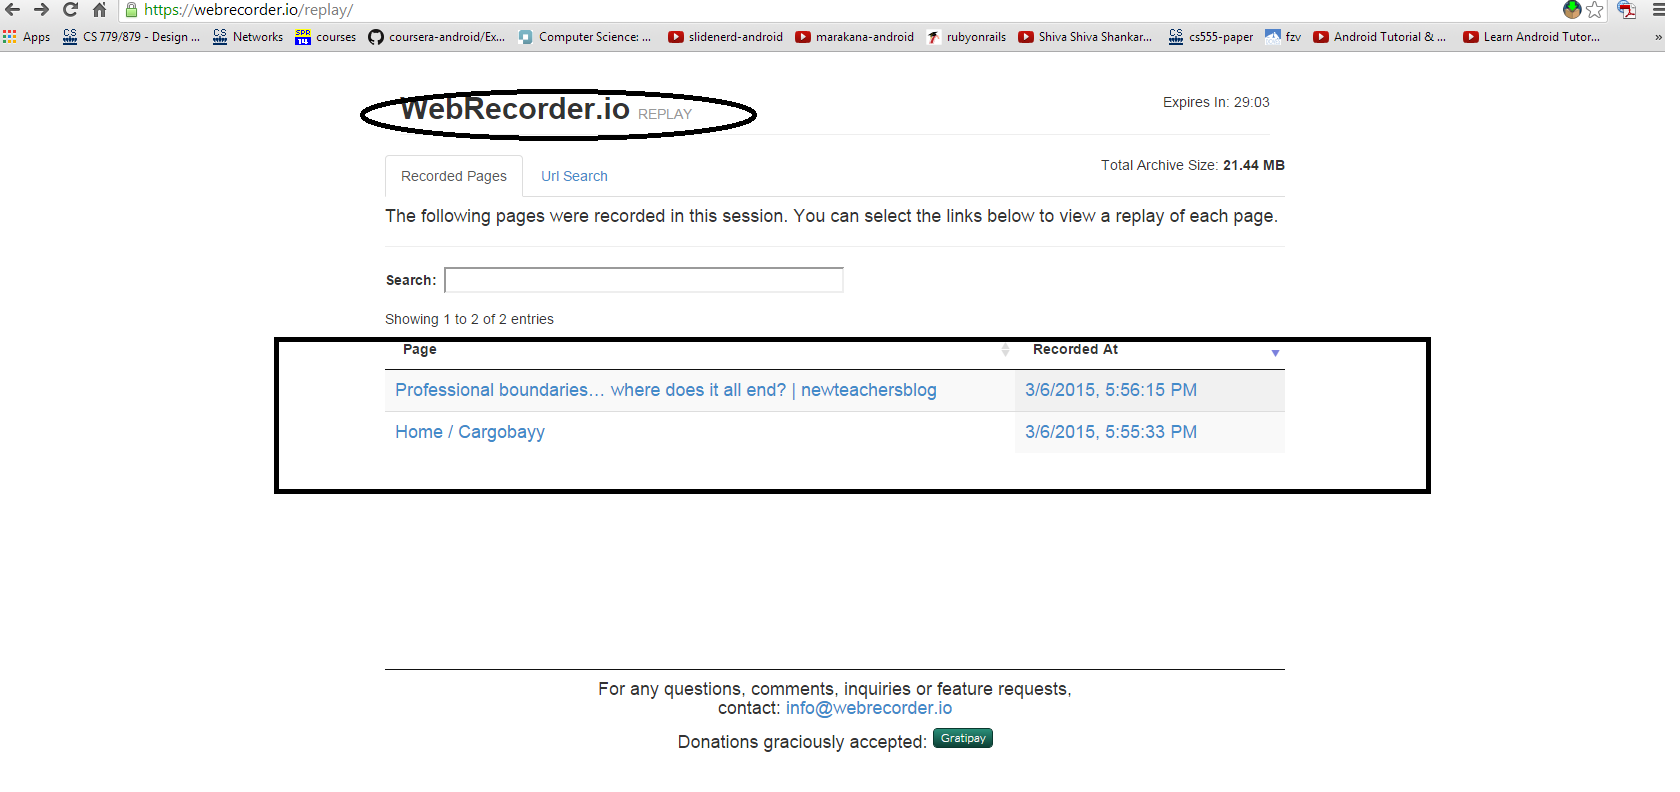
\includegraphics[scale=0.60]{webrecorderio-replay.png}
        \caption{webrecorder}
        \label{webrecorder.io}
    \end{center}
\end{figure}
\newpage
\begin{figure}[ht]    
    \begin{center}
        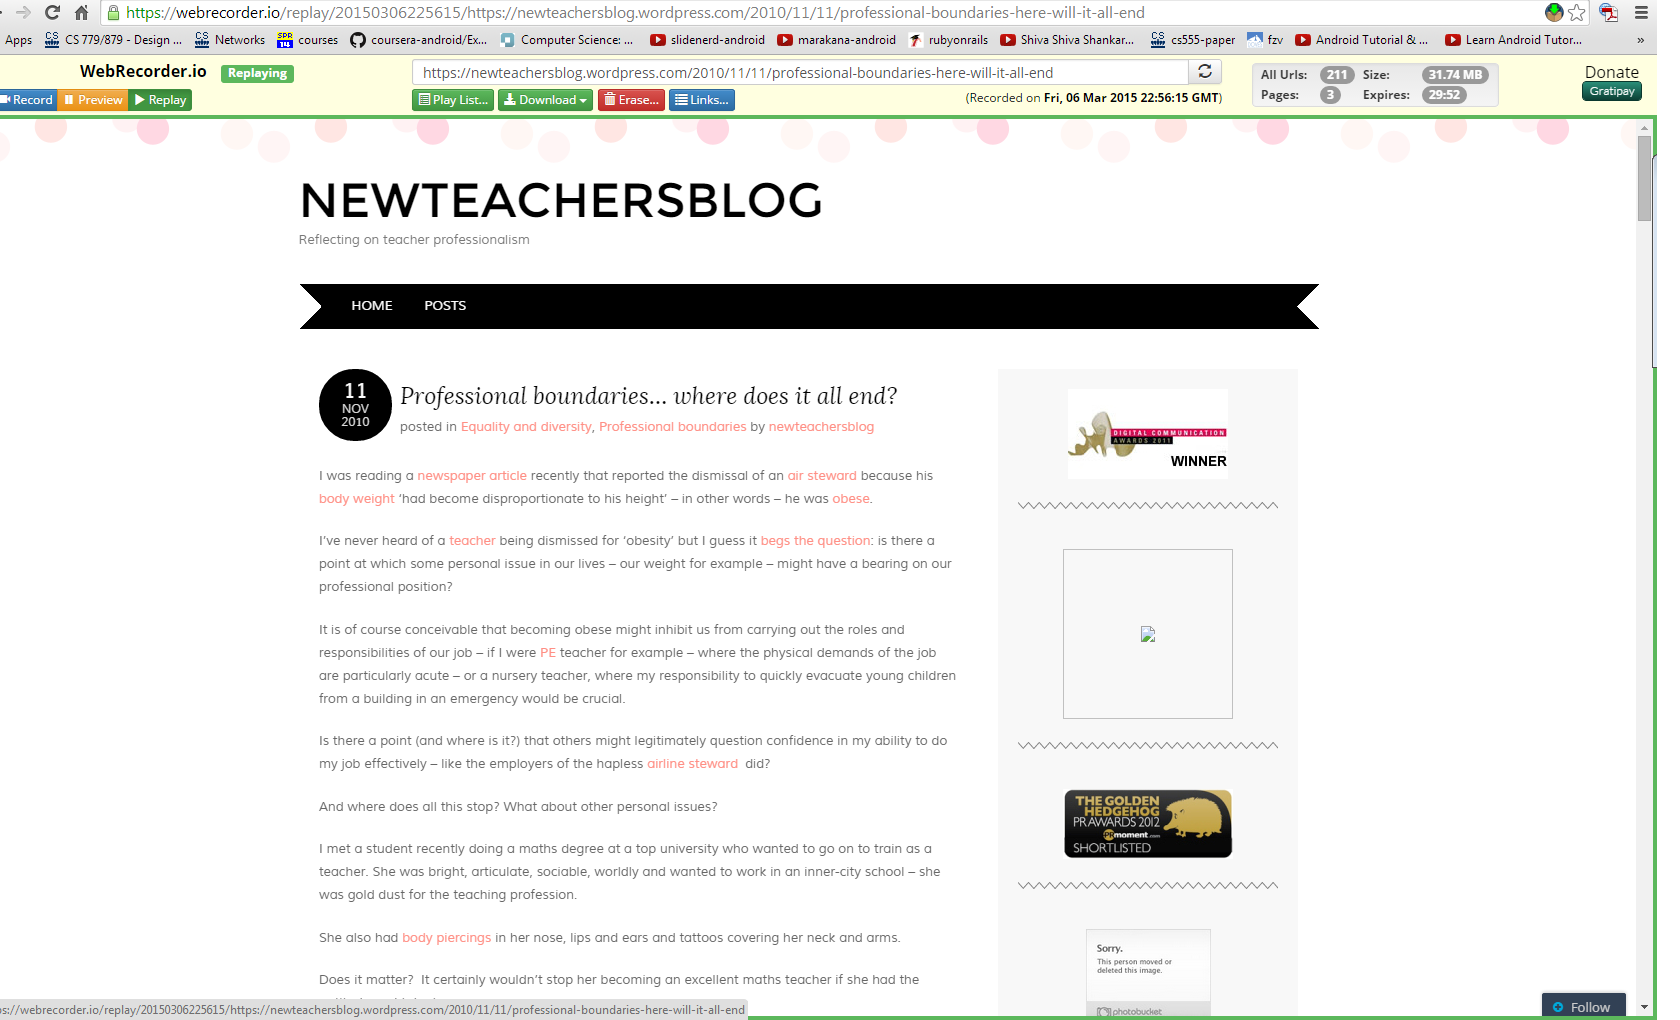
\includegraphics[scale=0.60]{webrecorderio-playbackfile1.png}
        \caption{webrecorder plaback file}
        \label{webrecorder playback}
    \end{center}
\end{figure}
\newpage


\newpage
\begin{figure}[ht]    
    \begin{center}
        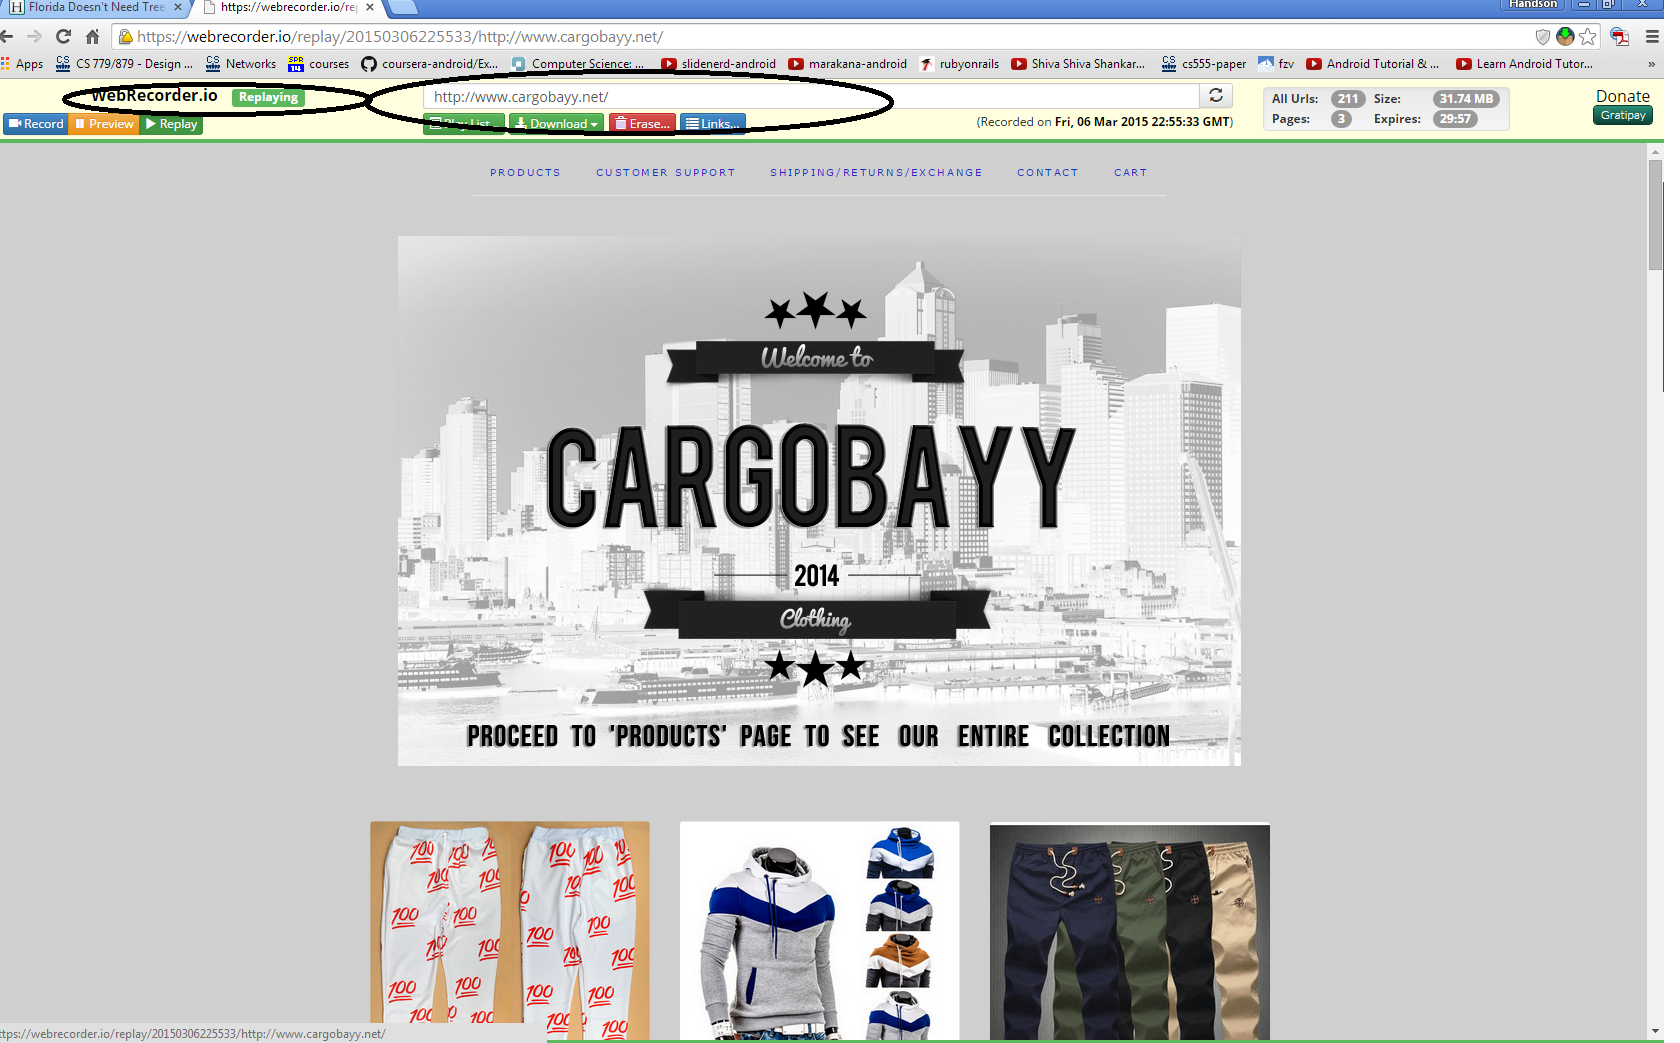
\includegraphics[scale=0.60]{webrecorderio-playbackfile2.png}
        \caption{webrecorder playback file 2}
        \label{webrecorder playback}
    \end{center}
\end{figure}
\newpage
  
  
\section{Part 2}

\paragraph{Ingest the 100 URIs from their resulting WARC files into a SOLR instance
see the code + tutorial at: https://github.com/ukwa/webarchive-discovery 
Demonstrate several functioning queries on the files (a full front-end is not required)
describe the configuration choices you made in setting up SOLR and processing the documents\\
}
  
  I have set up SOLR instance using the link ''https://github.com/ukwa/webarchive-discovery '' \\
  
  The pre-requisites for this are Maven 3 and Oracle java 7 .\\
  
  Following are the commands used to run SOLR instance.\\
    $ cd warc-solr-test-server \\
$ mvn jetty:run-exploded \\

This will fire up a suitable Solr instance, with a UI on port 8080 .

Indexing a WARC file \\

Downloaded warc-indexer from ''https://oss.sonatype.org/content/repositories/snapshots/uk/bl/wa/discovery/warc-indexer/2.0.1-SNAPSHOT/'' \\

Copied the downloaded folder to webdiscovery. \\

Merged all the 100 WARC files using the WARC merger posted in google groups. \\


Indexed the warc file using the command  \\

--java -jar warc-indexer-2.0.1-SNAPSHOT-jar-with-dependencies.jar  -s http://localhost:8080/discovery -t warc-indexer/src/test/resources/wikipedia-mona-lisa/flashfrozen-jwat-recompressed.warc.gz



\subparagraph{Querying SOLR}

The queries i have used are \\

1  To search the host name using xml content , change host name data changes automatically (shown in the figure 9  ,17\\

2 To get json data , set up wt to json (shown in figure 10  ) \\

3 To get xml data , set up wt to xml (shown in figure 16 ) \\

4 To retrieve only two rows from the query , set up  row count to 2 (shown in figure  16) \\

5 To search based on host name in json script(shown in figure 10 )\\



\newpage
\begin{figure}[ht]    
    \begin{center}
        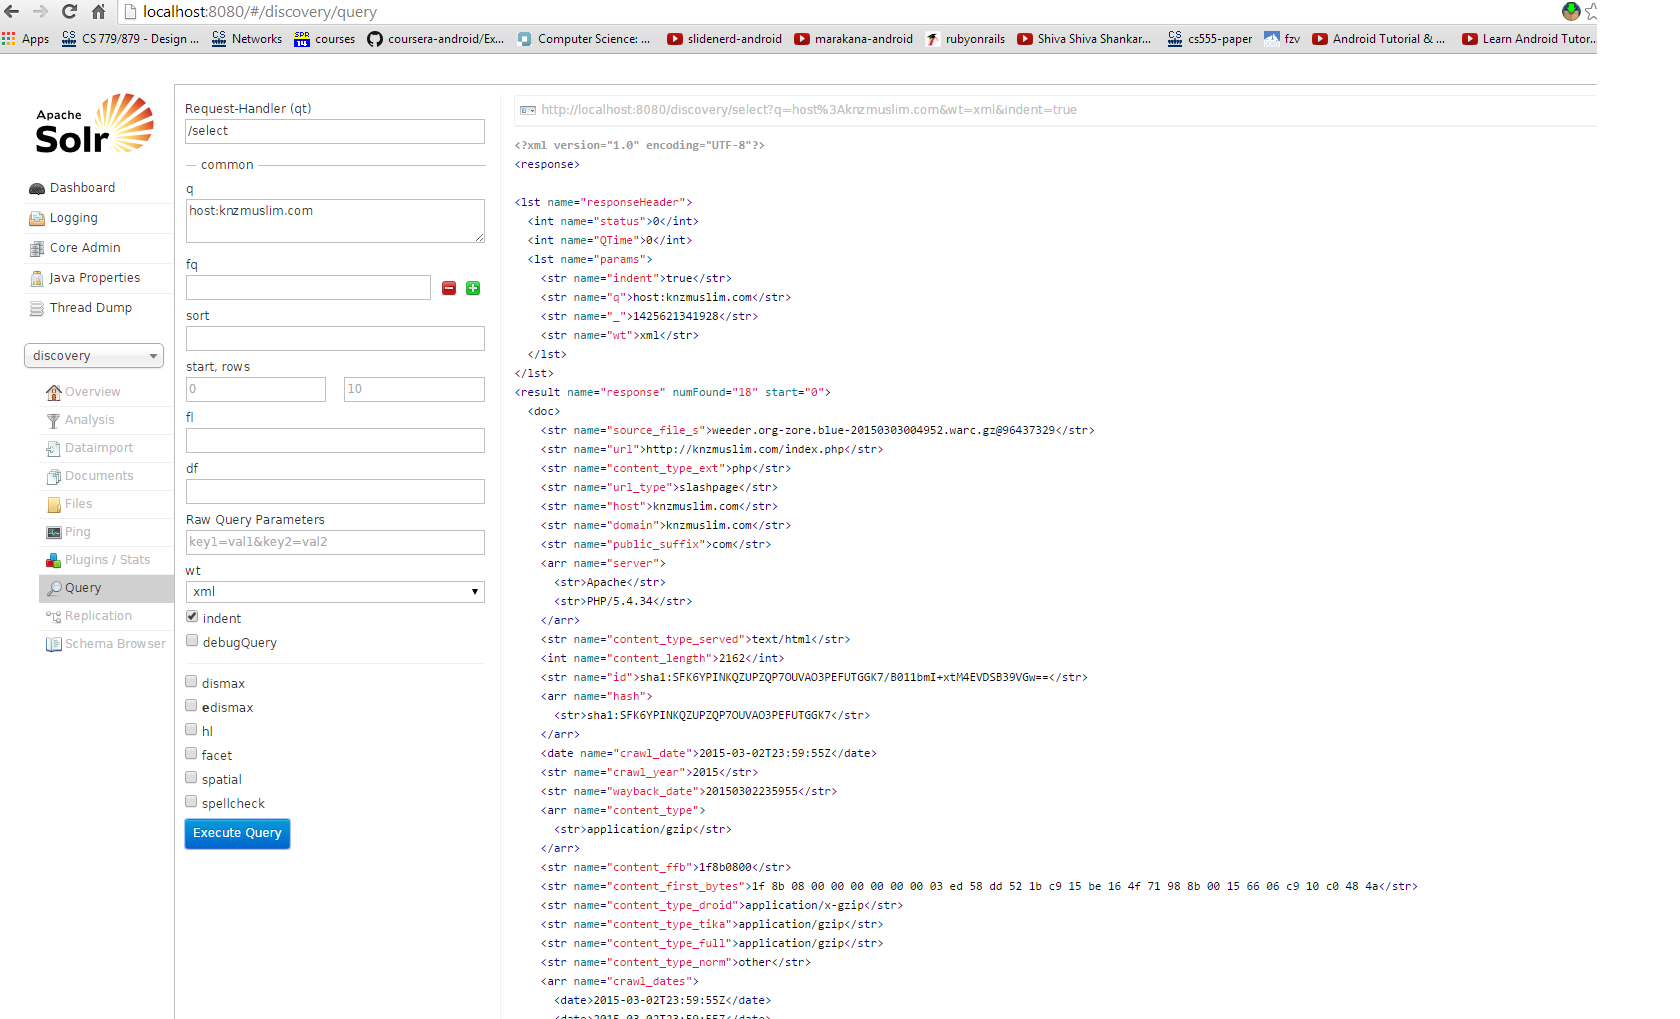
\includegraphics[scale=0.60]{hostname-xmlsearch.png}
        \caption{Querying solrInstance }
        \label{Querying SOLR}
    \end{center}
\end{figure}
\newpage




  \newpage
\begin{figure}[ht]    
    \begin{center}
        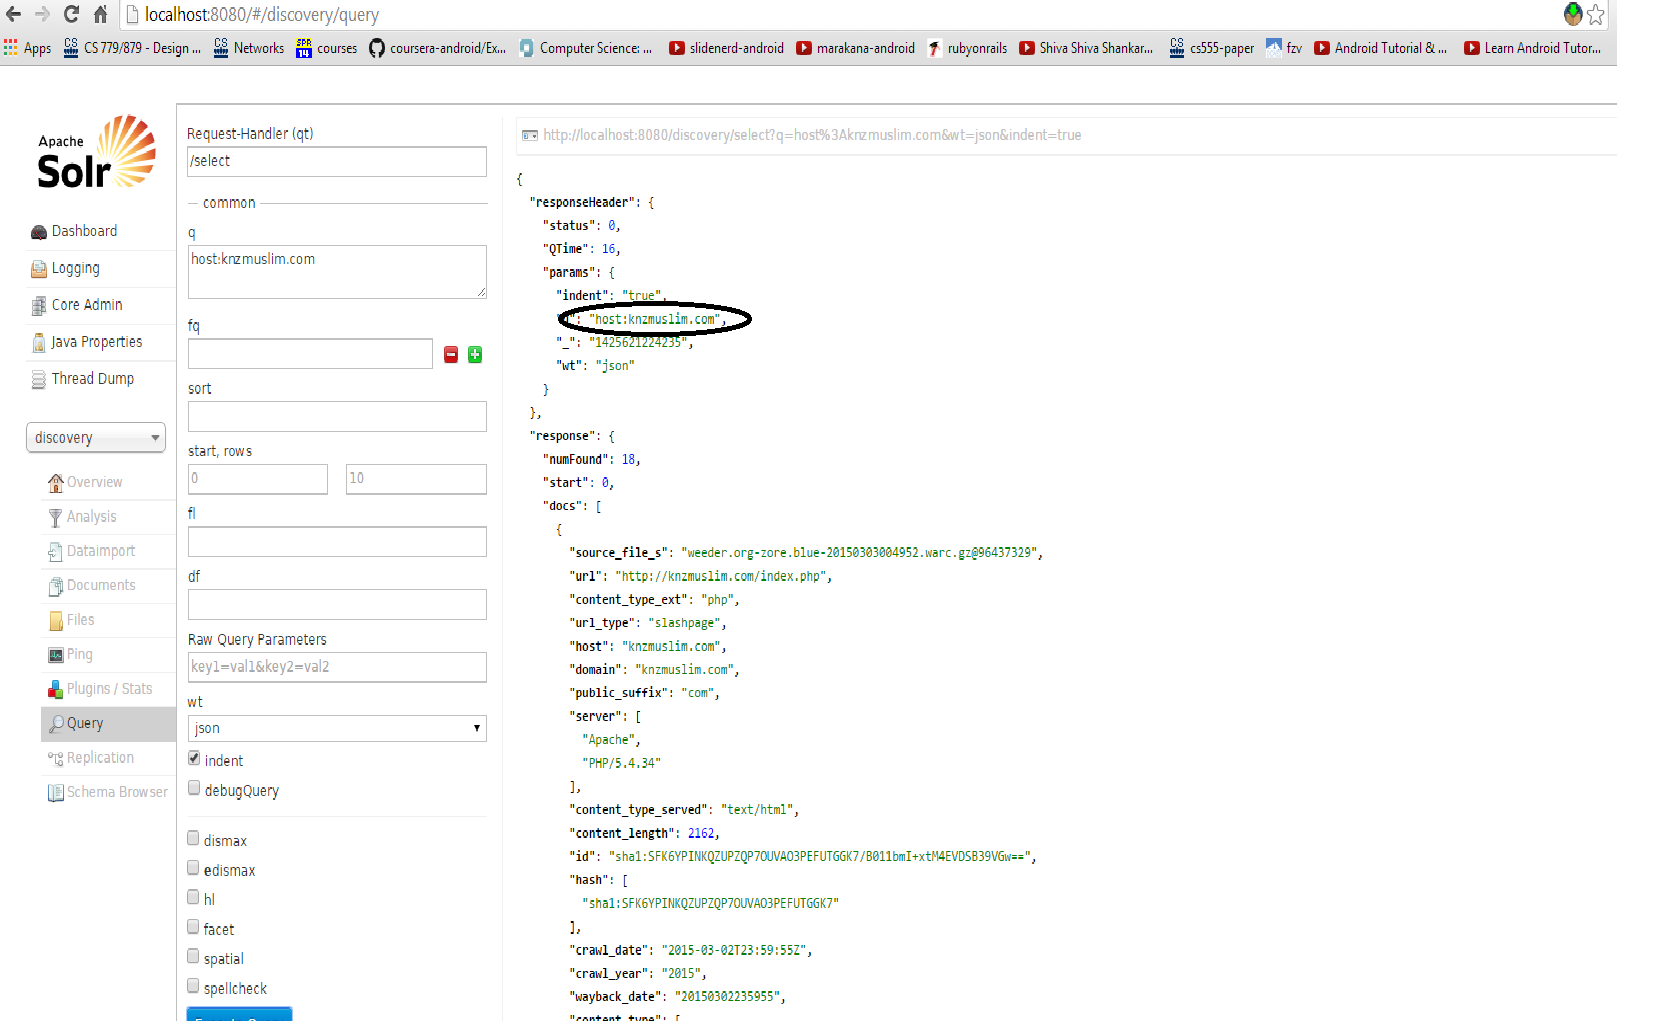
\includegraphics[scale=0.60]{changeinhostname.png}
        \caption{Querying solrInstance }
        \label{Querying SOLR}
    \end{center}
\end{figure}
\newpage


    \newpage
\begin{figure}[ht]    
    \begin{center}
        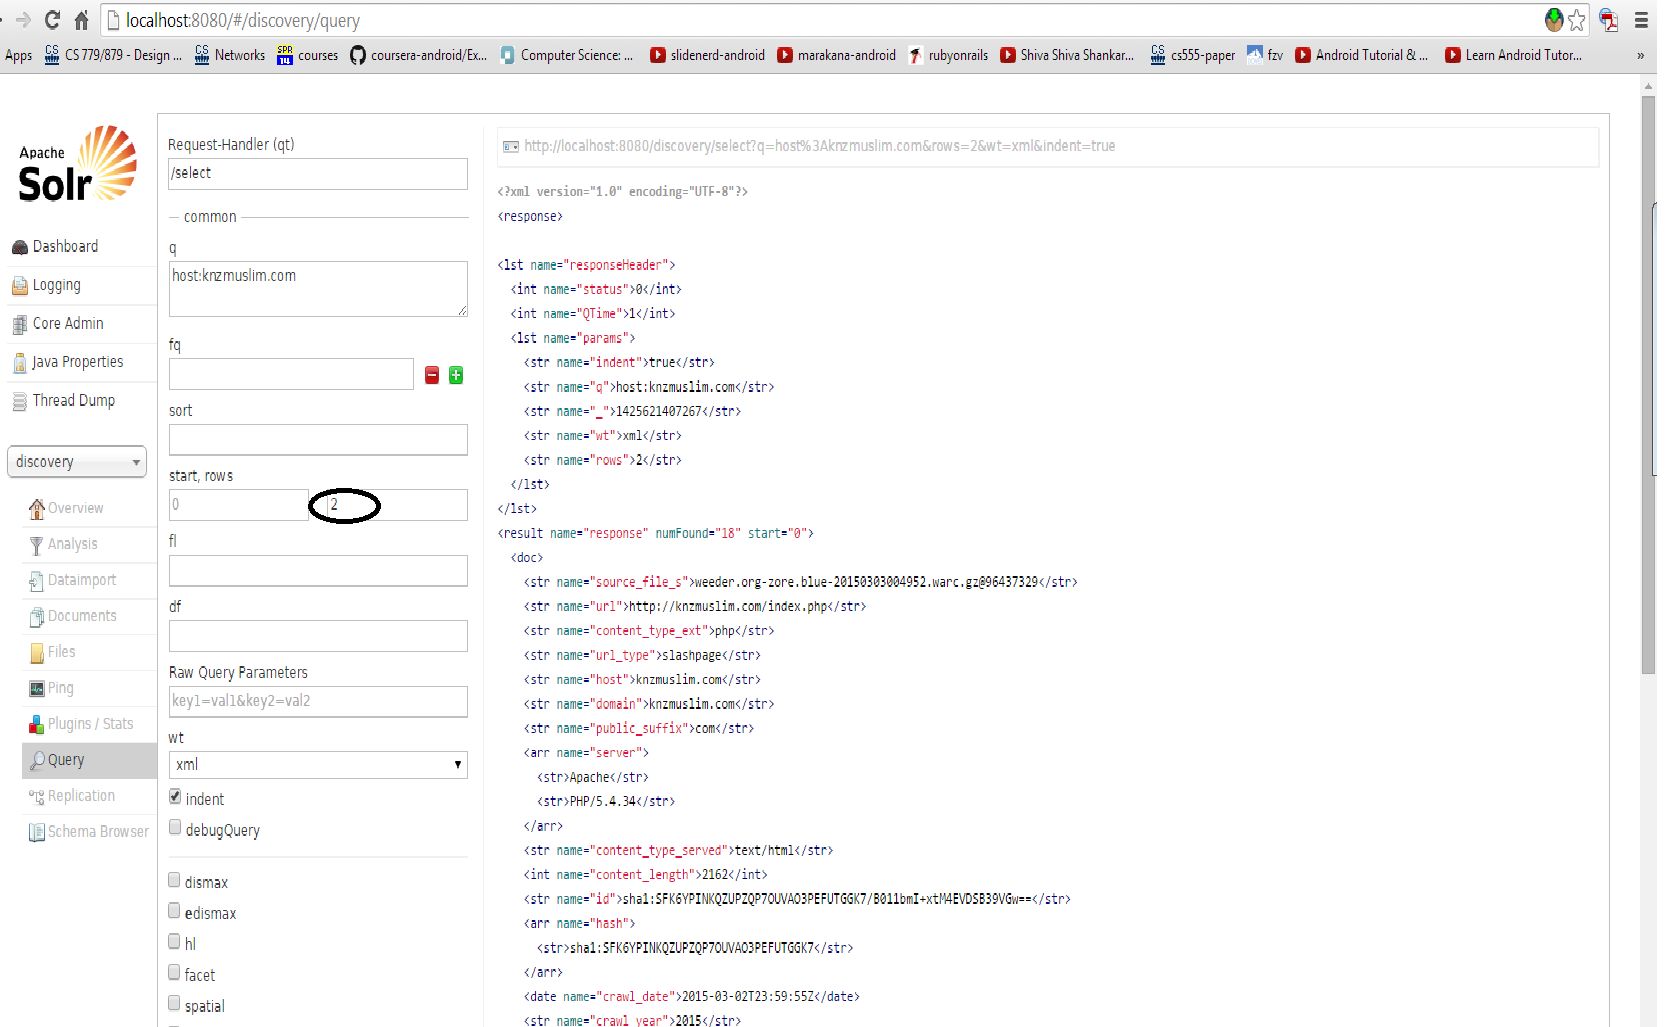
\includegraphics[scale=0.60]{noofrows.png}
        \caption{Querying solrInstance }
        \label{Querying SOLR}
    \end{center}
\end{figure}
\newpage
  
 
 
   \newpage
\begin{figure}[ht]    
    \begin{center}
        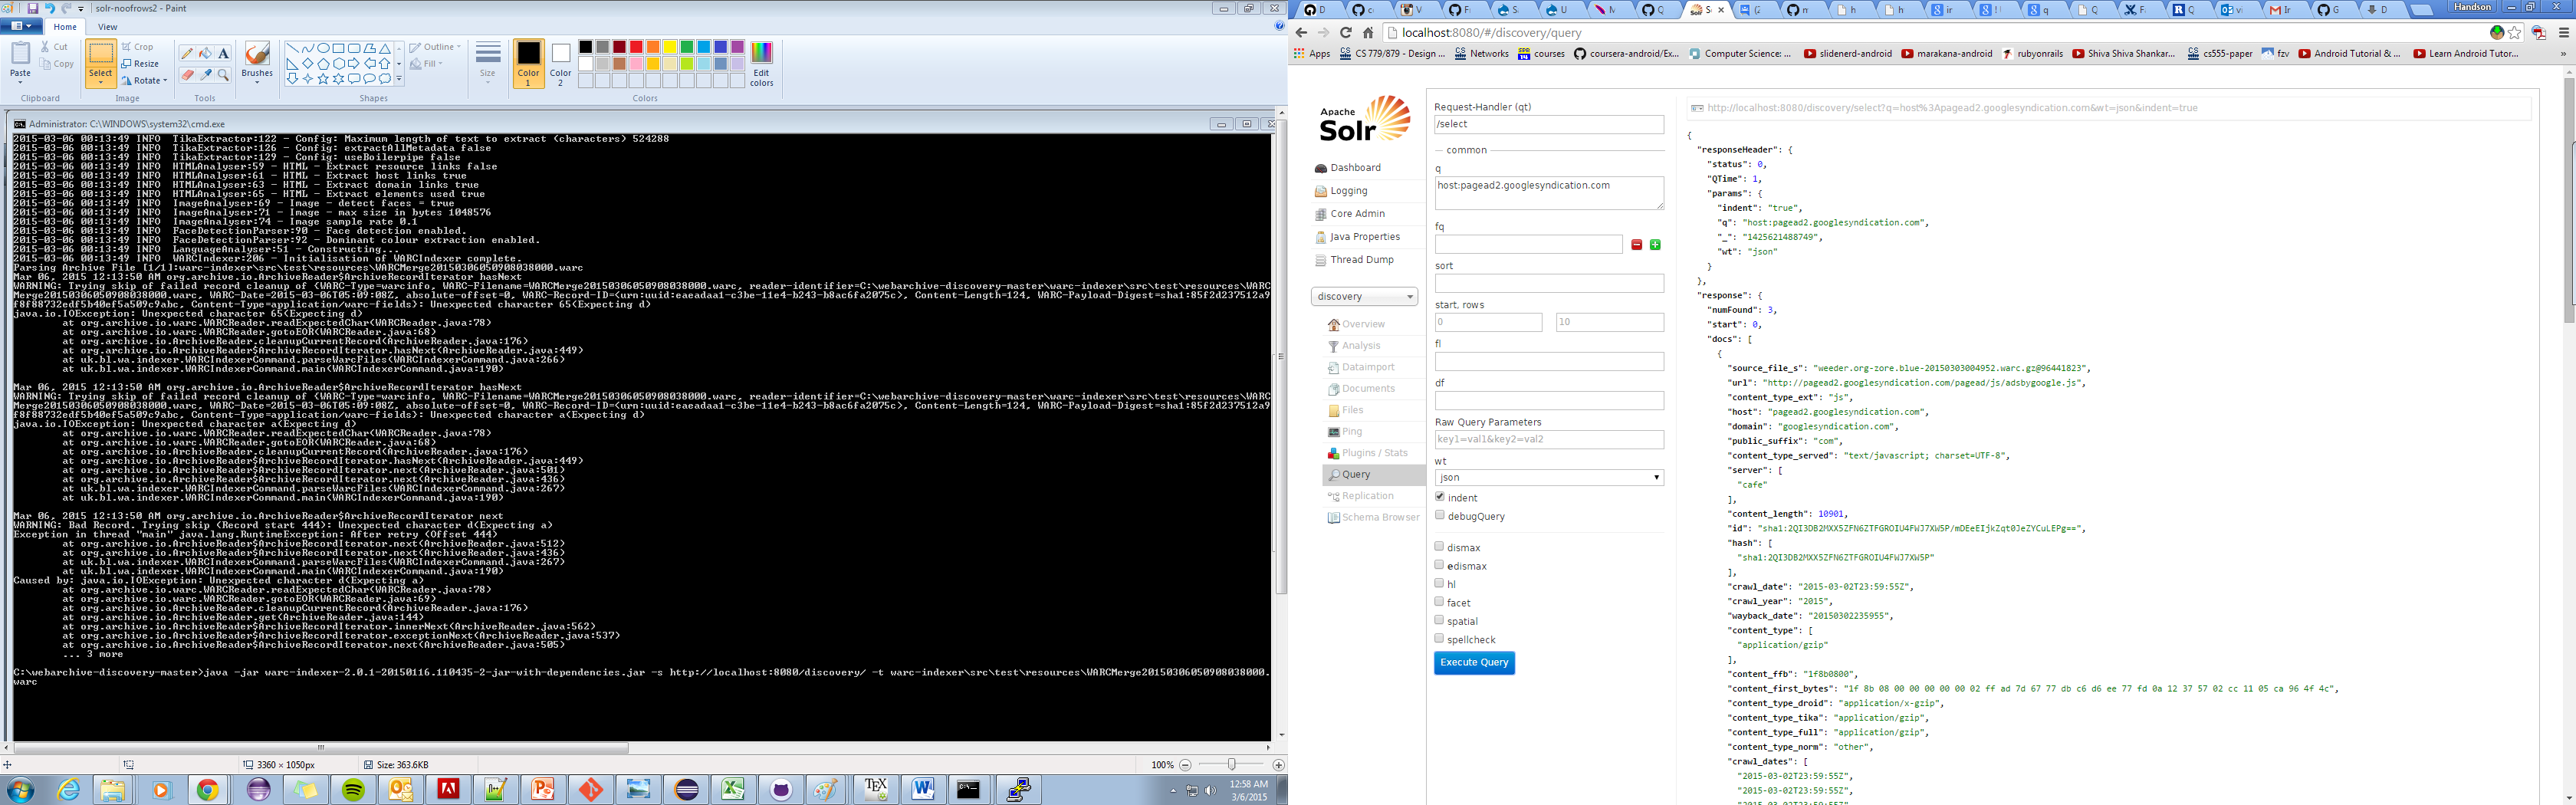
\includegraphics[scale=0.60]{solrchangeinhost.png}
        \caption{Querying solrInstance }
        \label{Querying SOLR}
    \end{center}
\end{figure}
\newpage


  
 
 
\end{document}



